\begin{figure}[H]
    \centering
    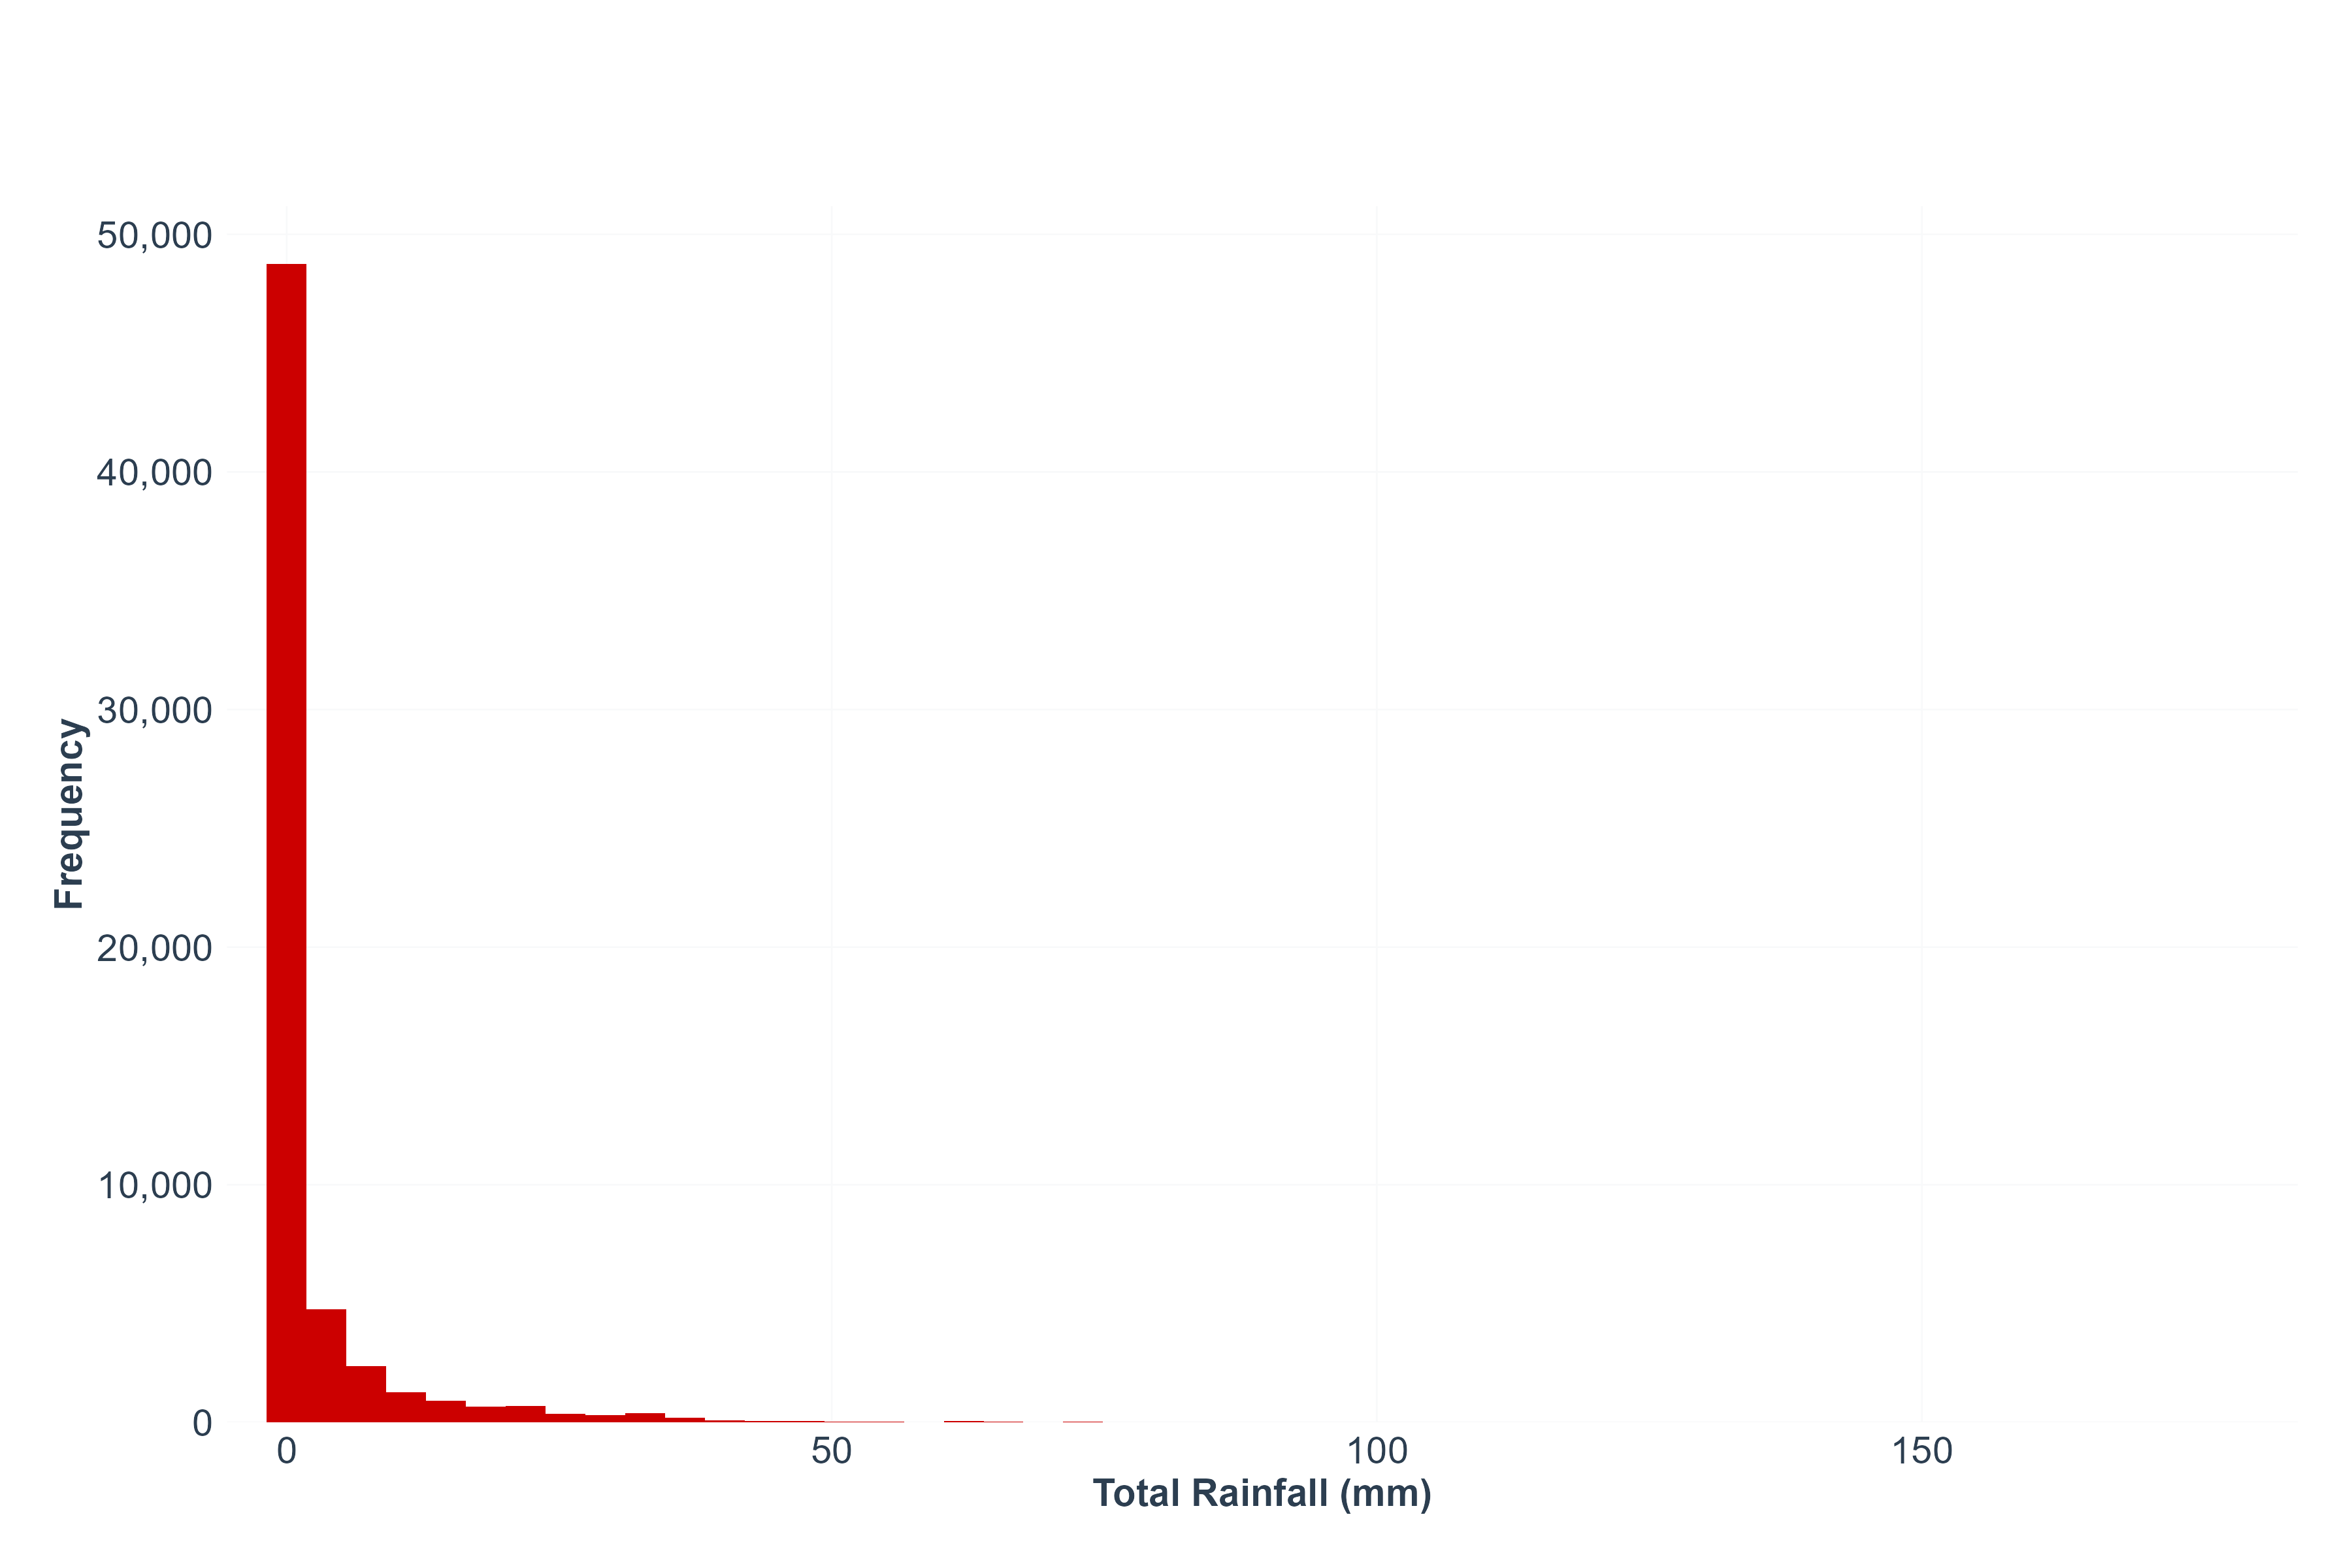
\includegraphics[width=0.8\textwidth]{../figures/rainfall_histogram.png}
    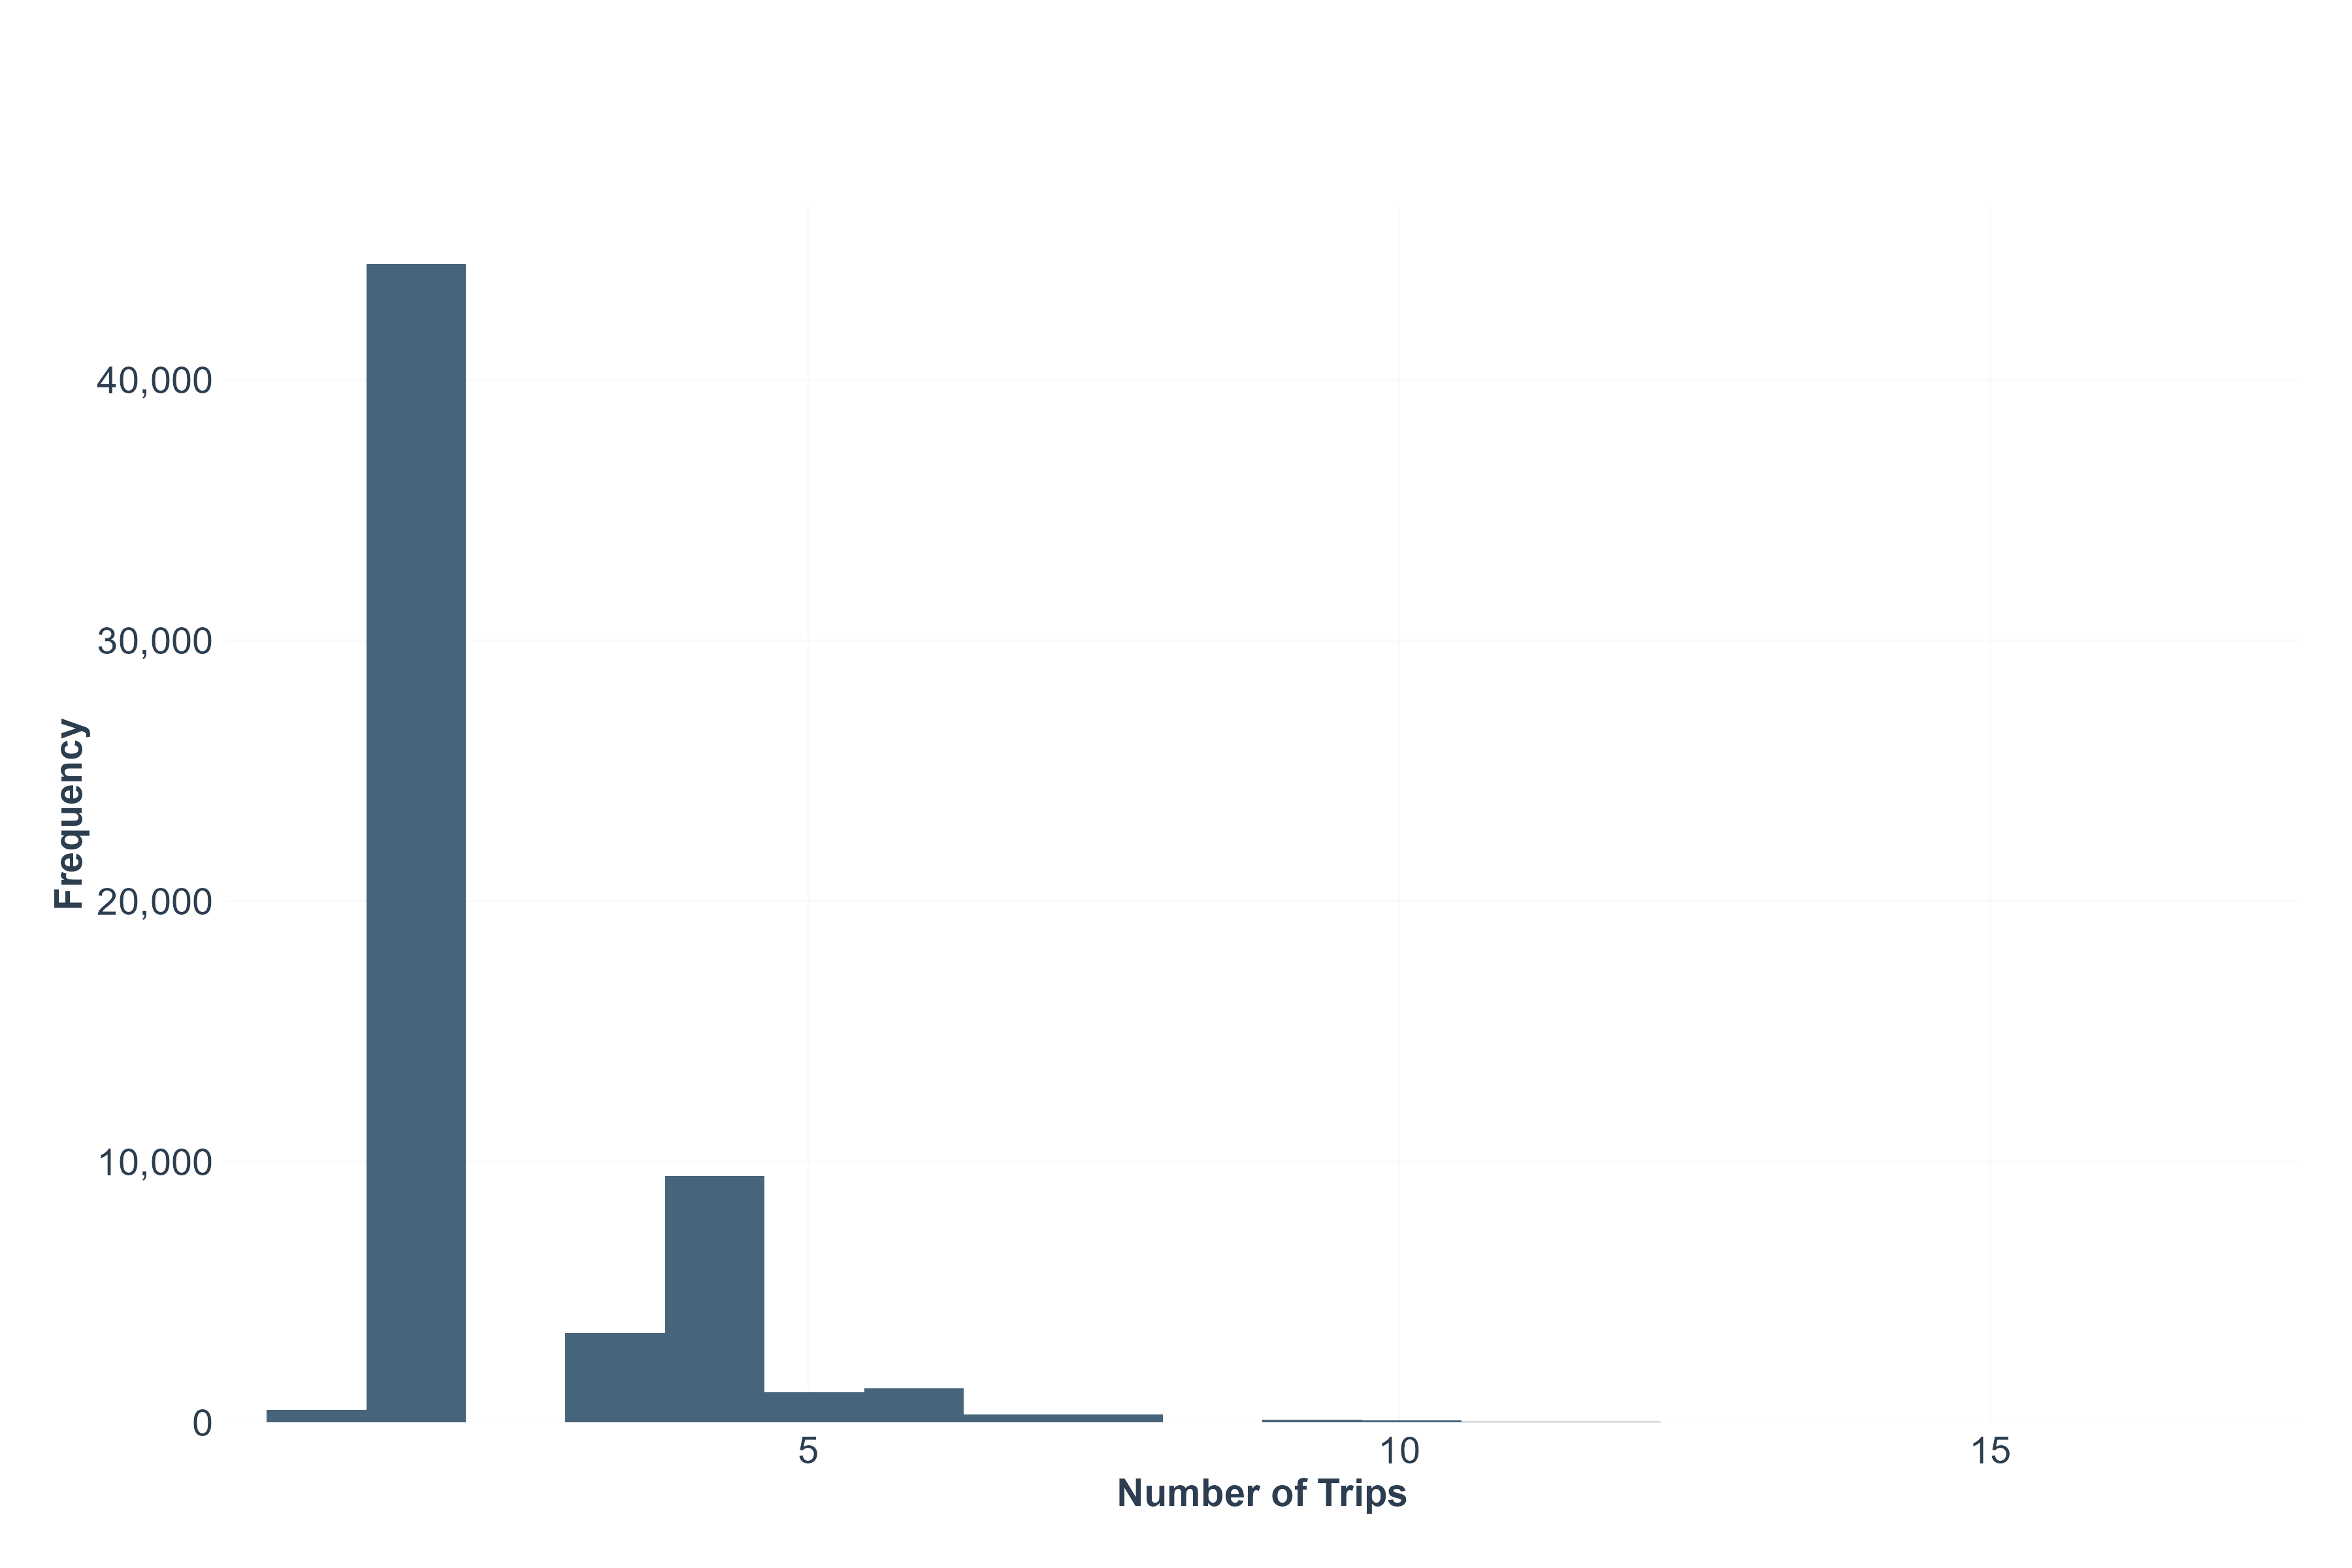
\includegraphics[width=0.8\textwidth]{../figures/trips_histogram.png}
    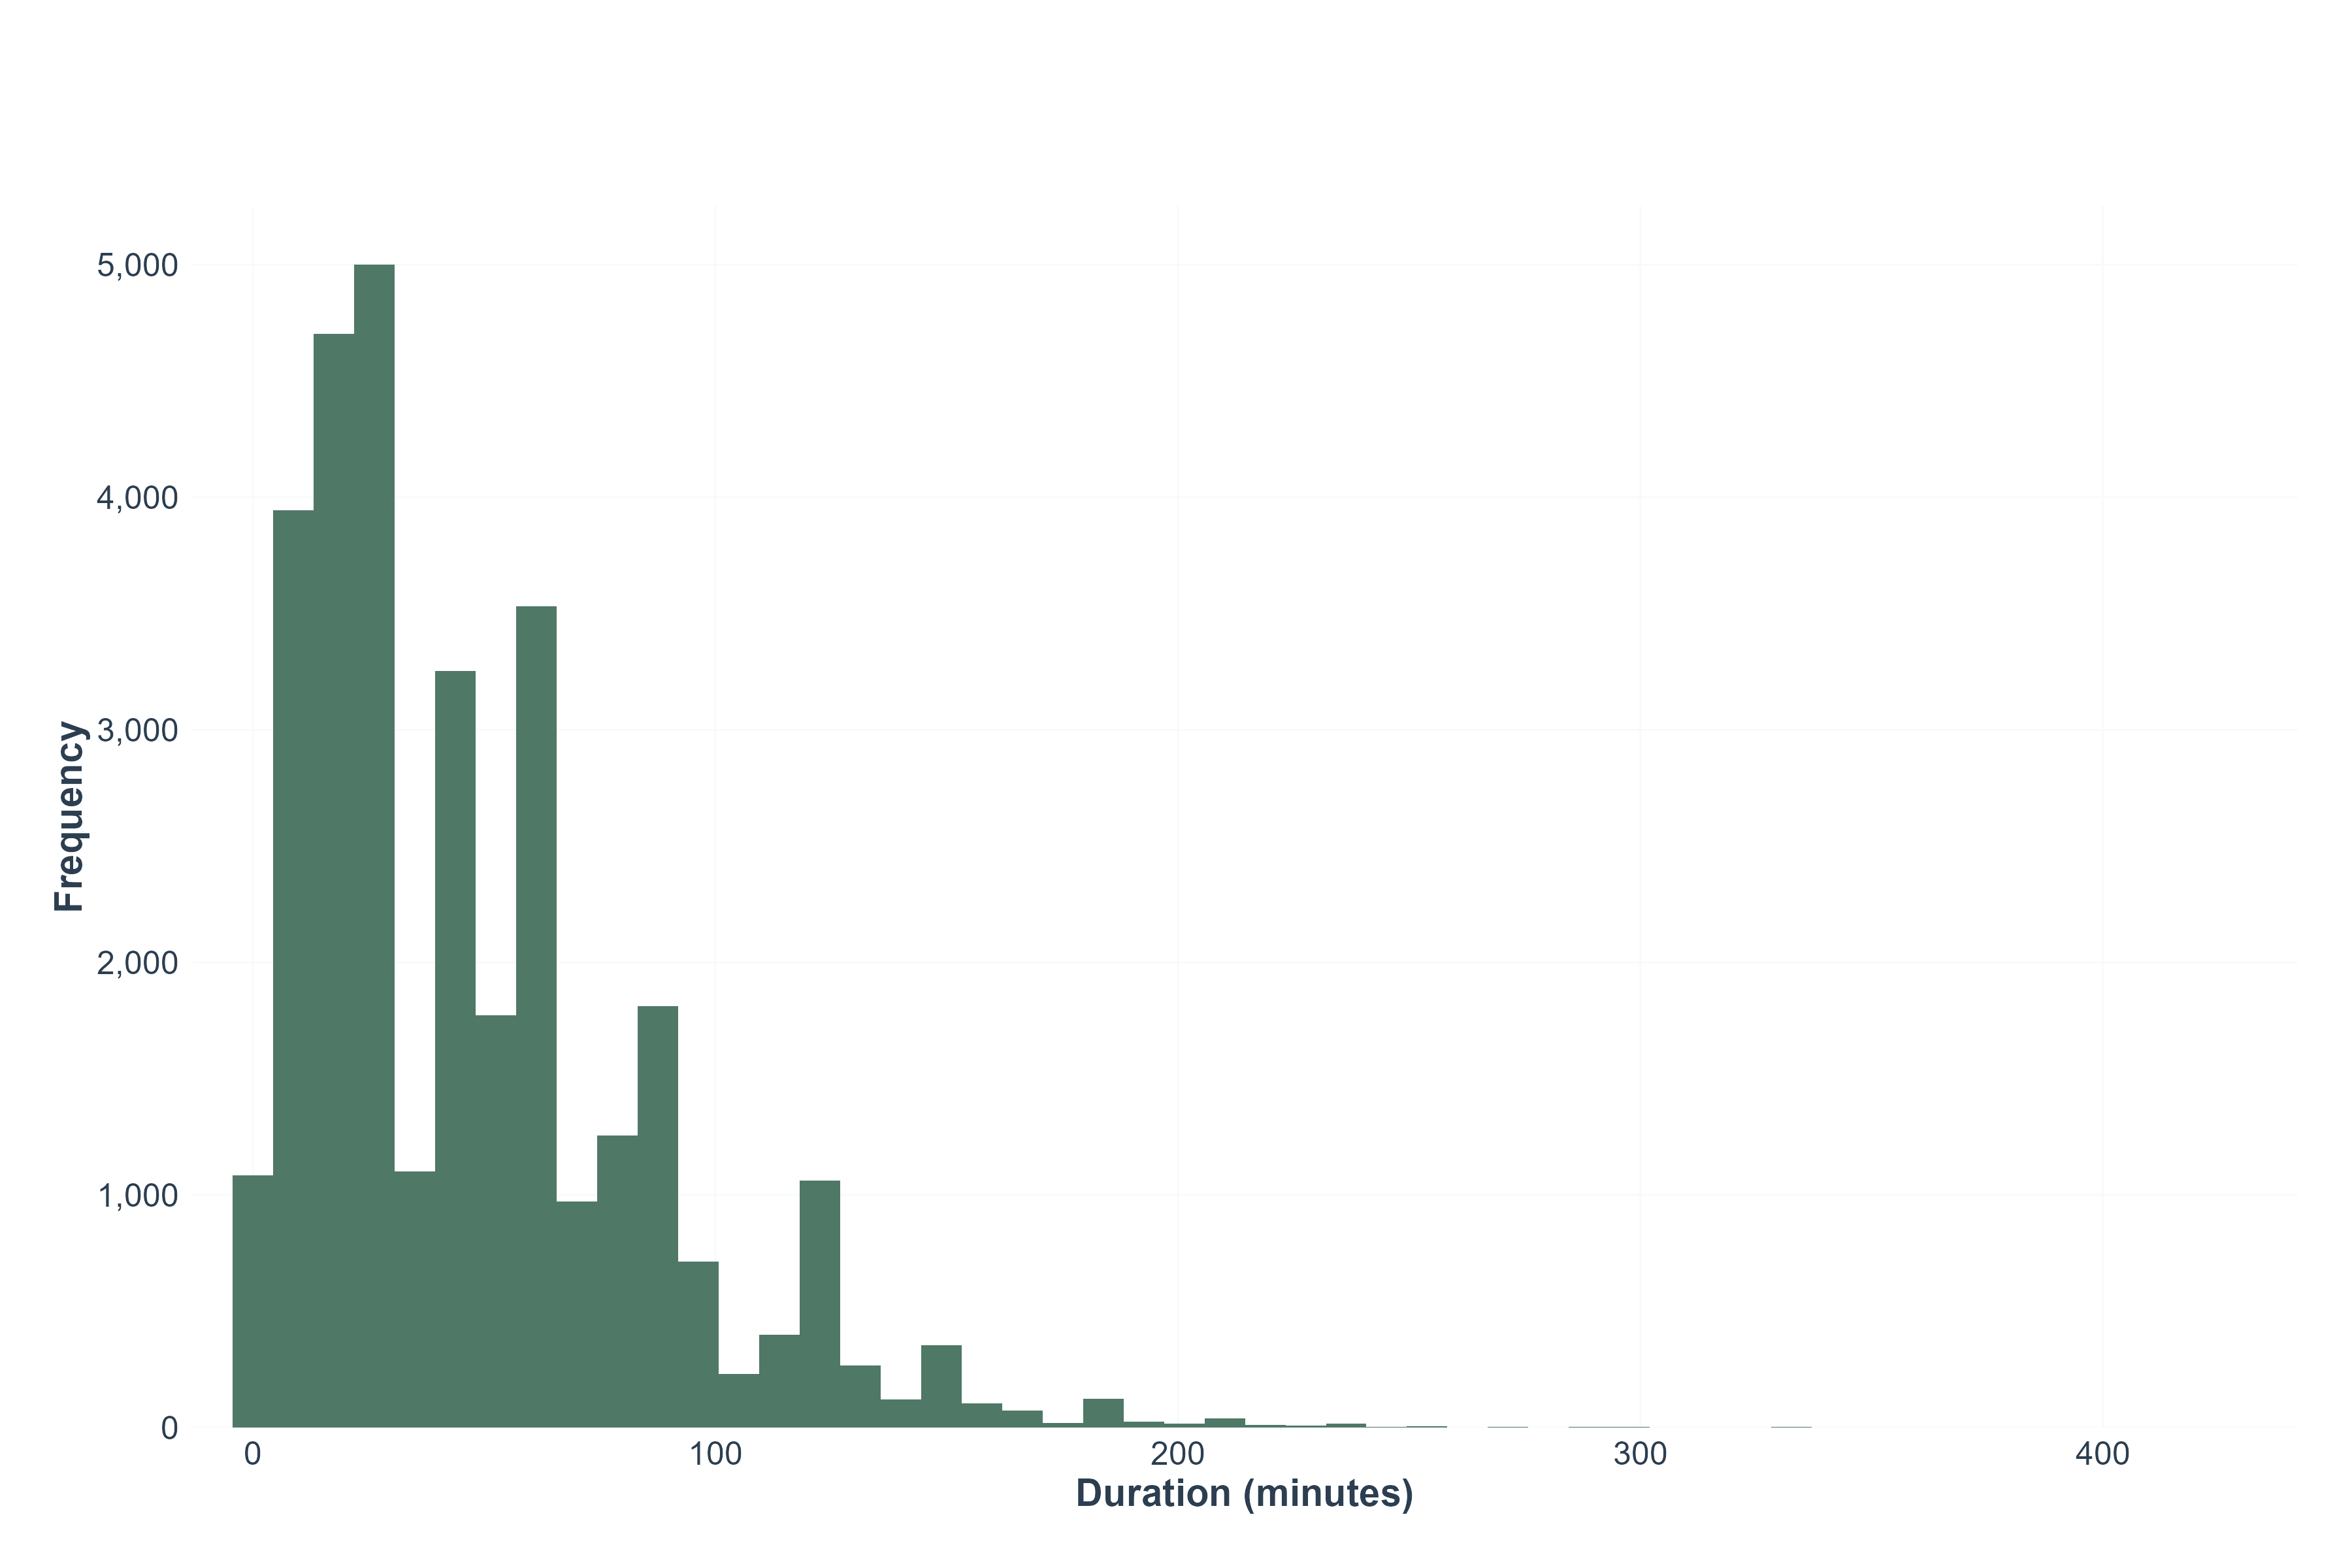
\includegraphics[width=0.8\textwidth]{../figures/duration_histogram.png}
    \caption{Histograms showing the distributions of rainfall (top), number of trips (middle), and trip durations (bottom) in the dataset.}
    \label{fig:hist}
\end{figure}

\begin{figure}[H]
    \centering
    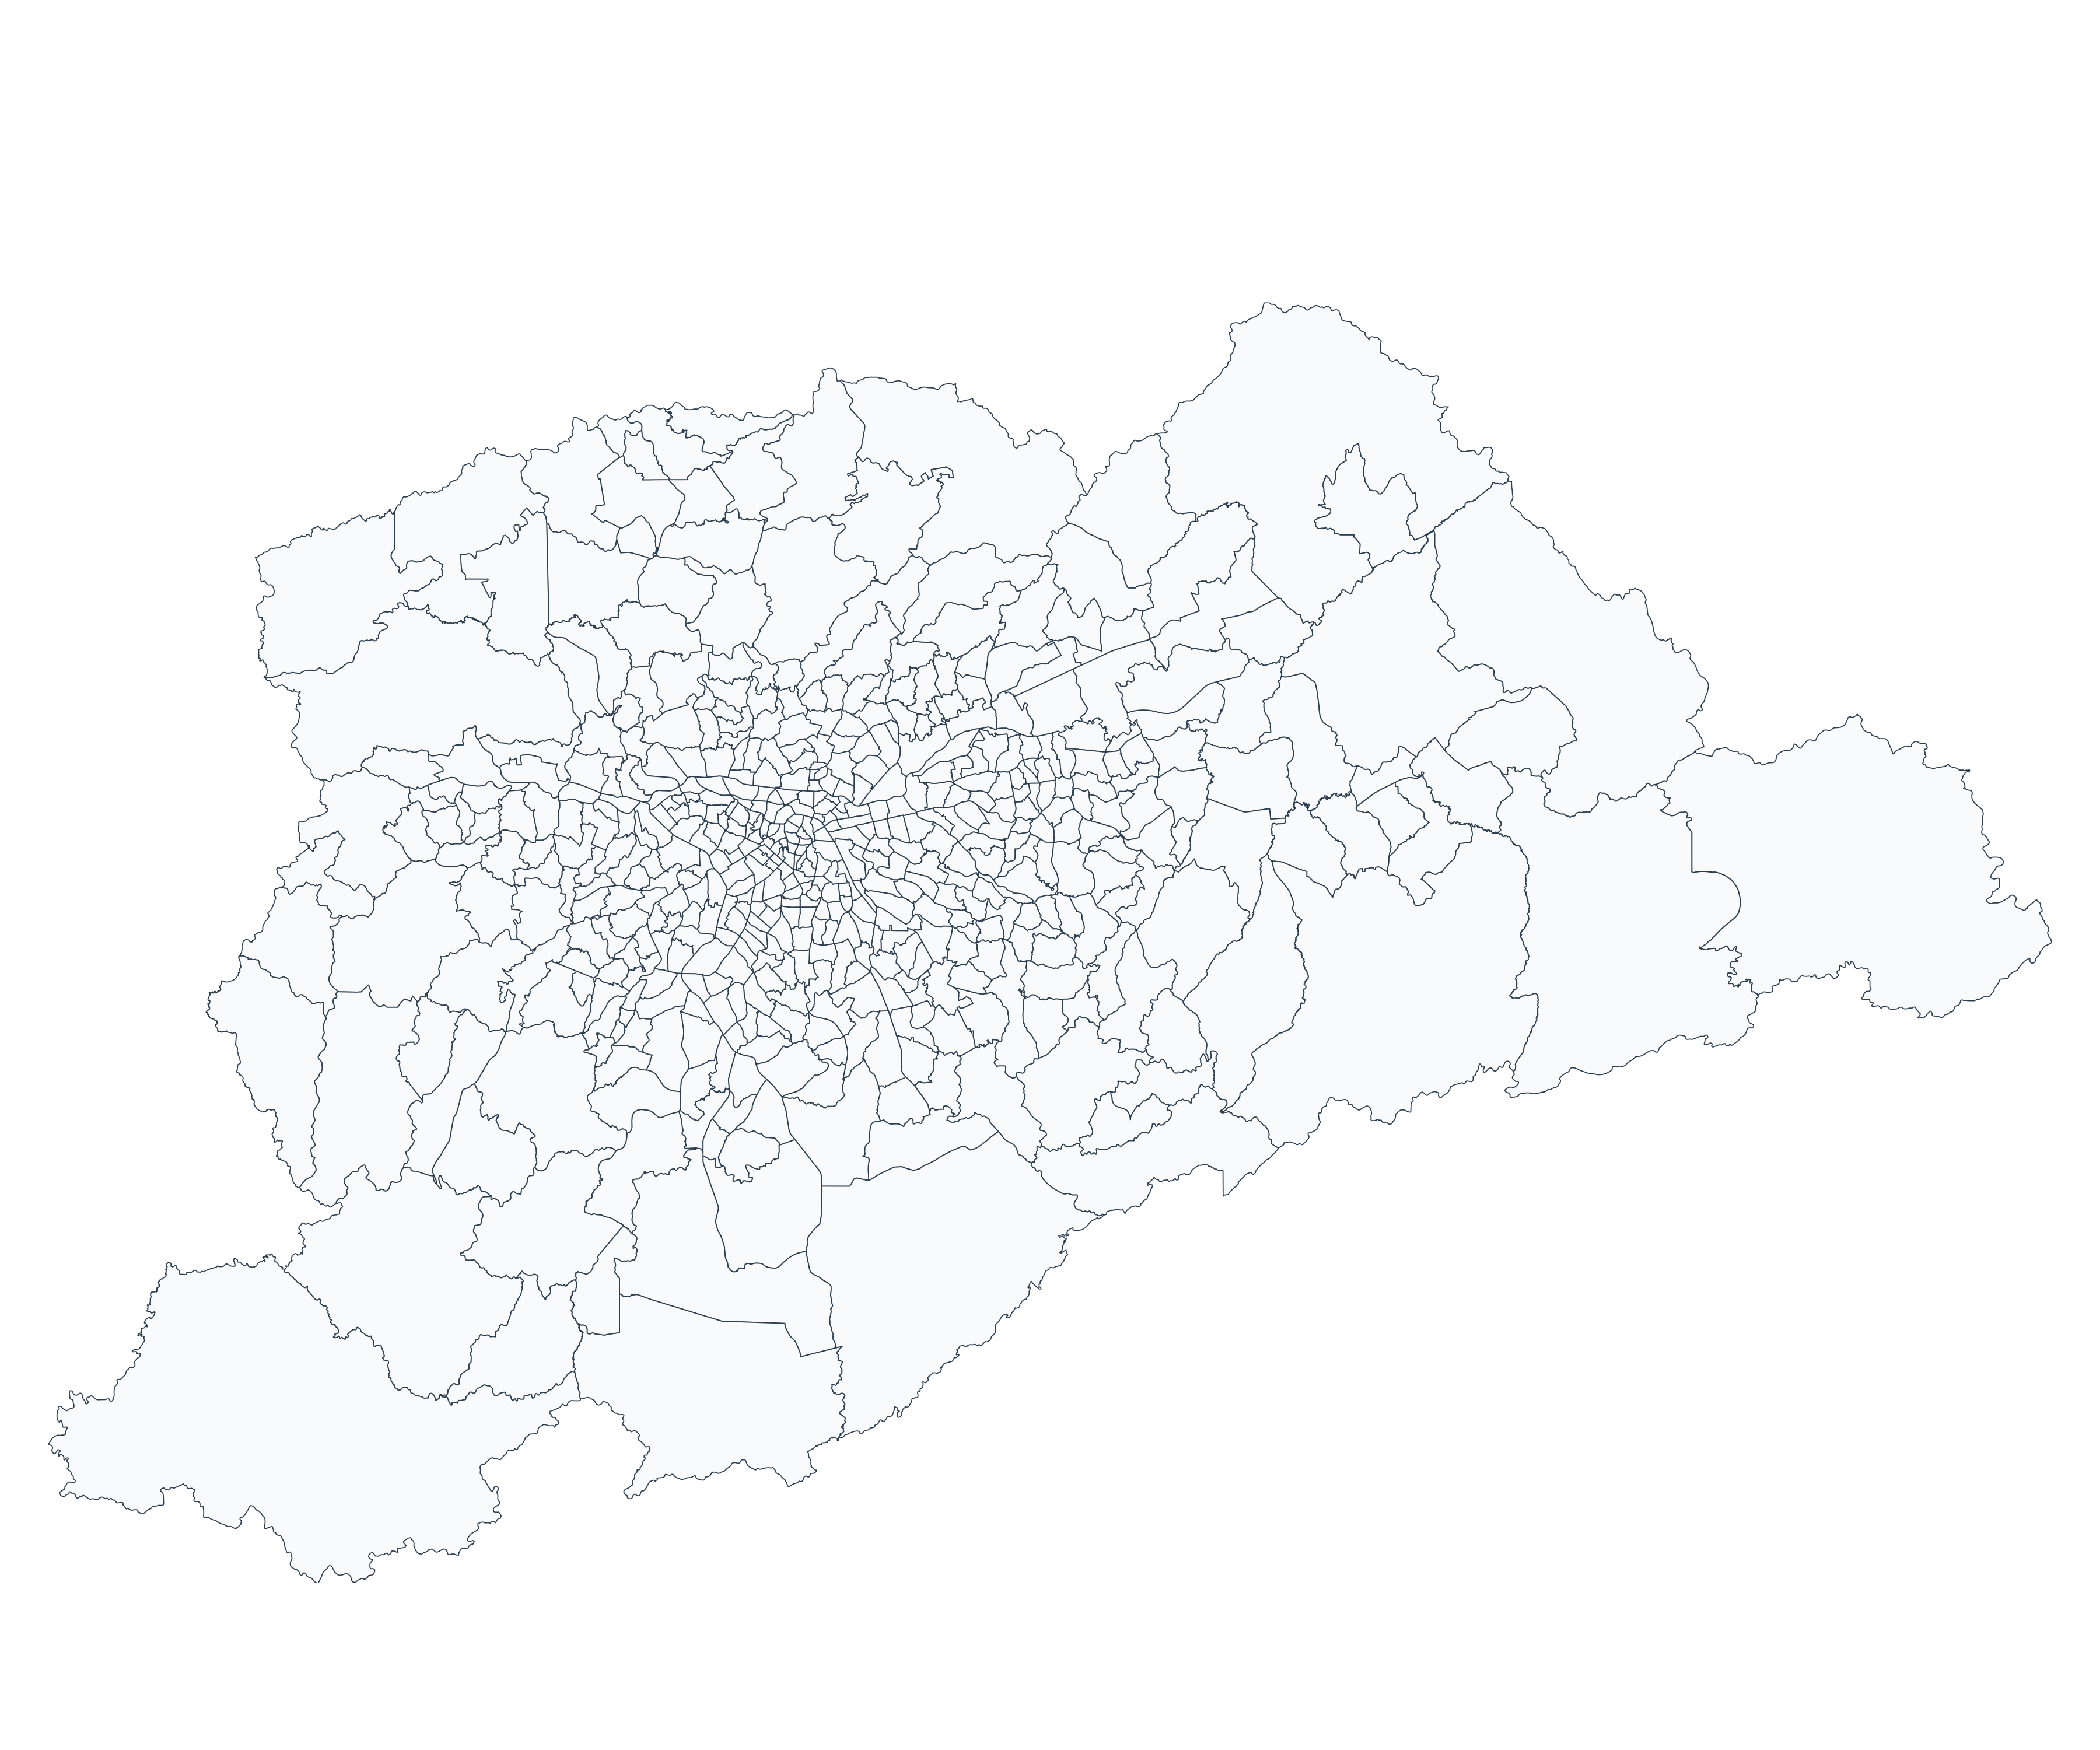
\includegraphics[width=0.8\textwidth]{../figures/rmsp_base.png}
    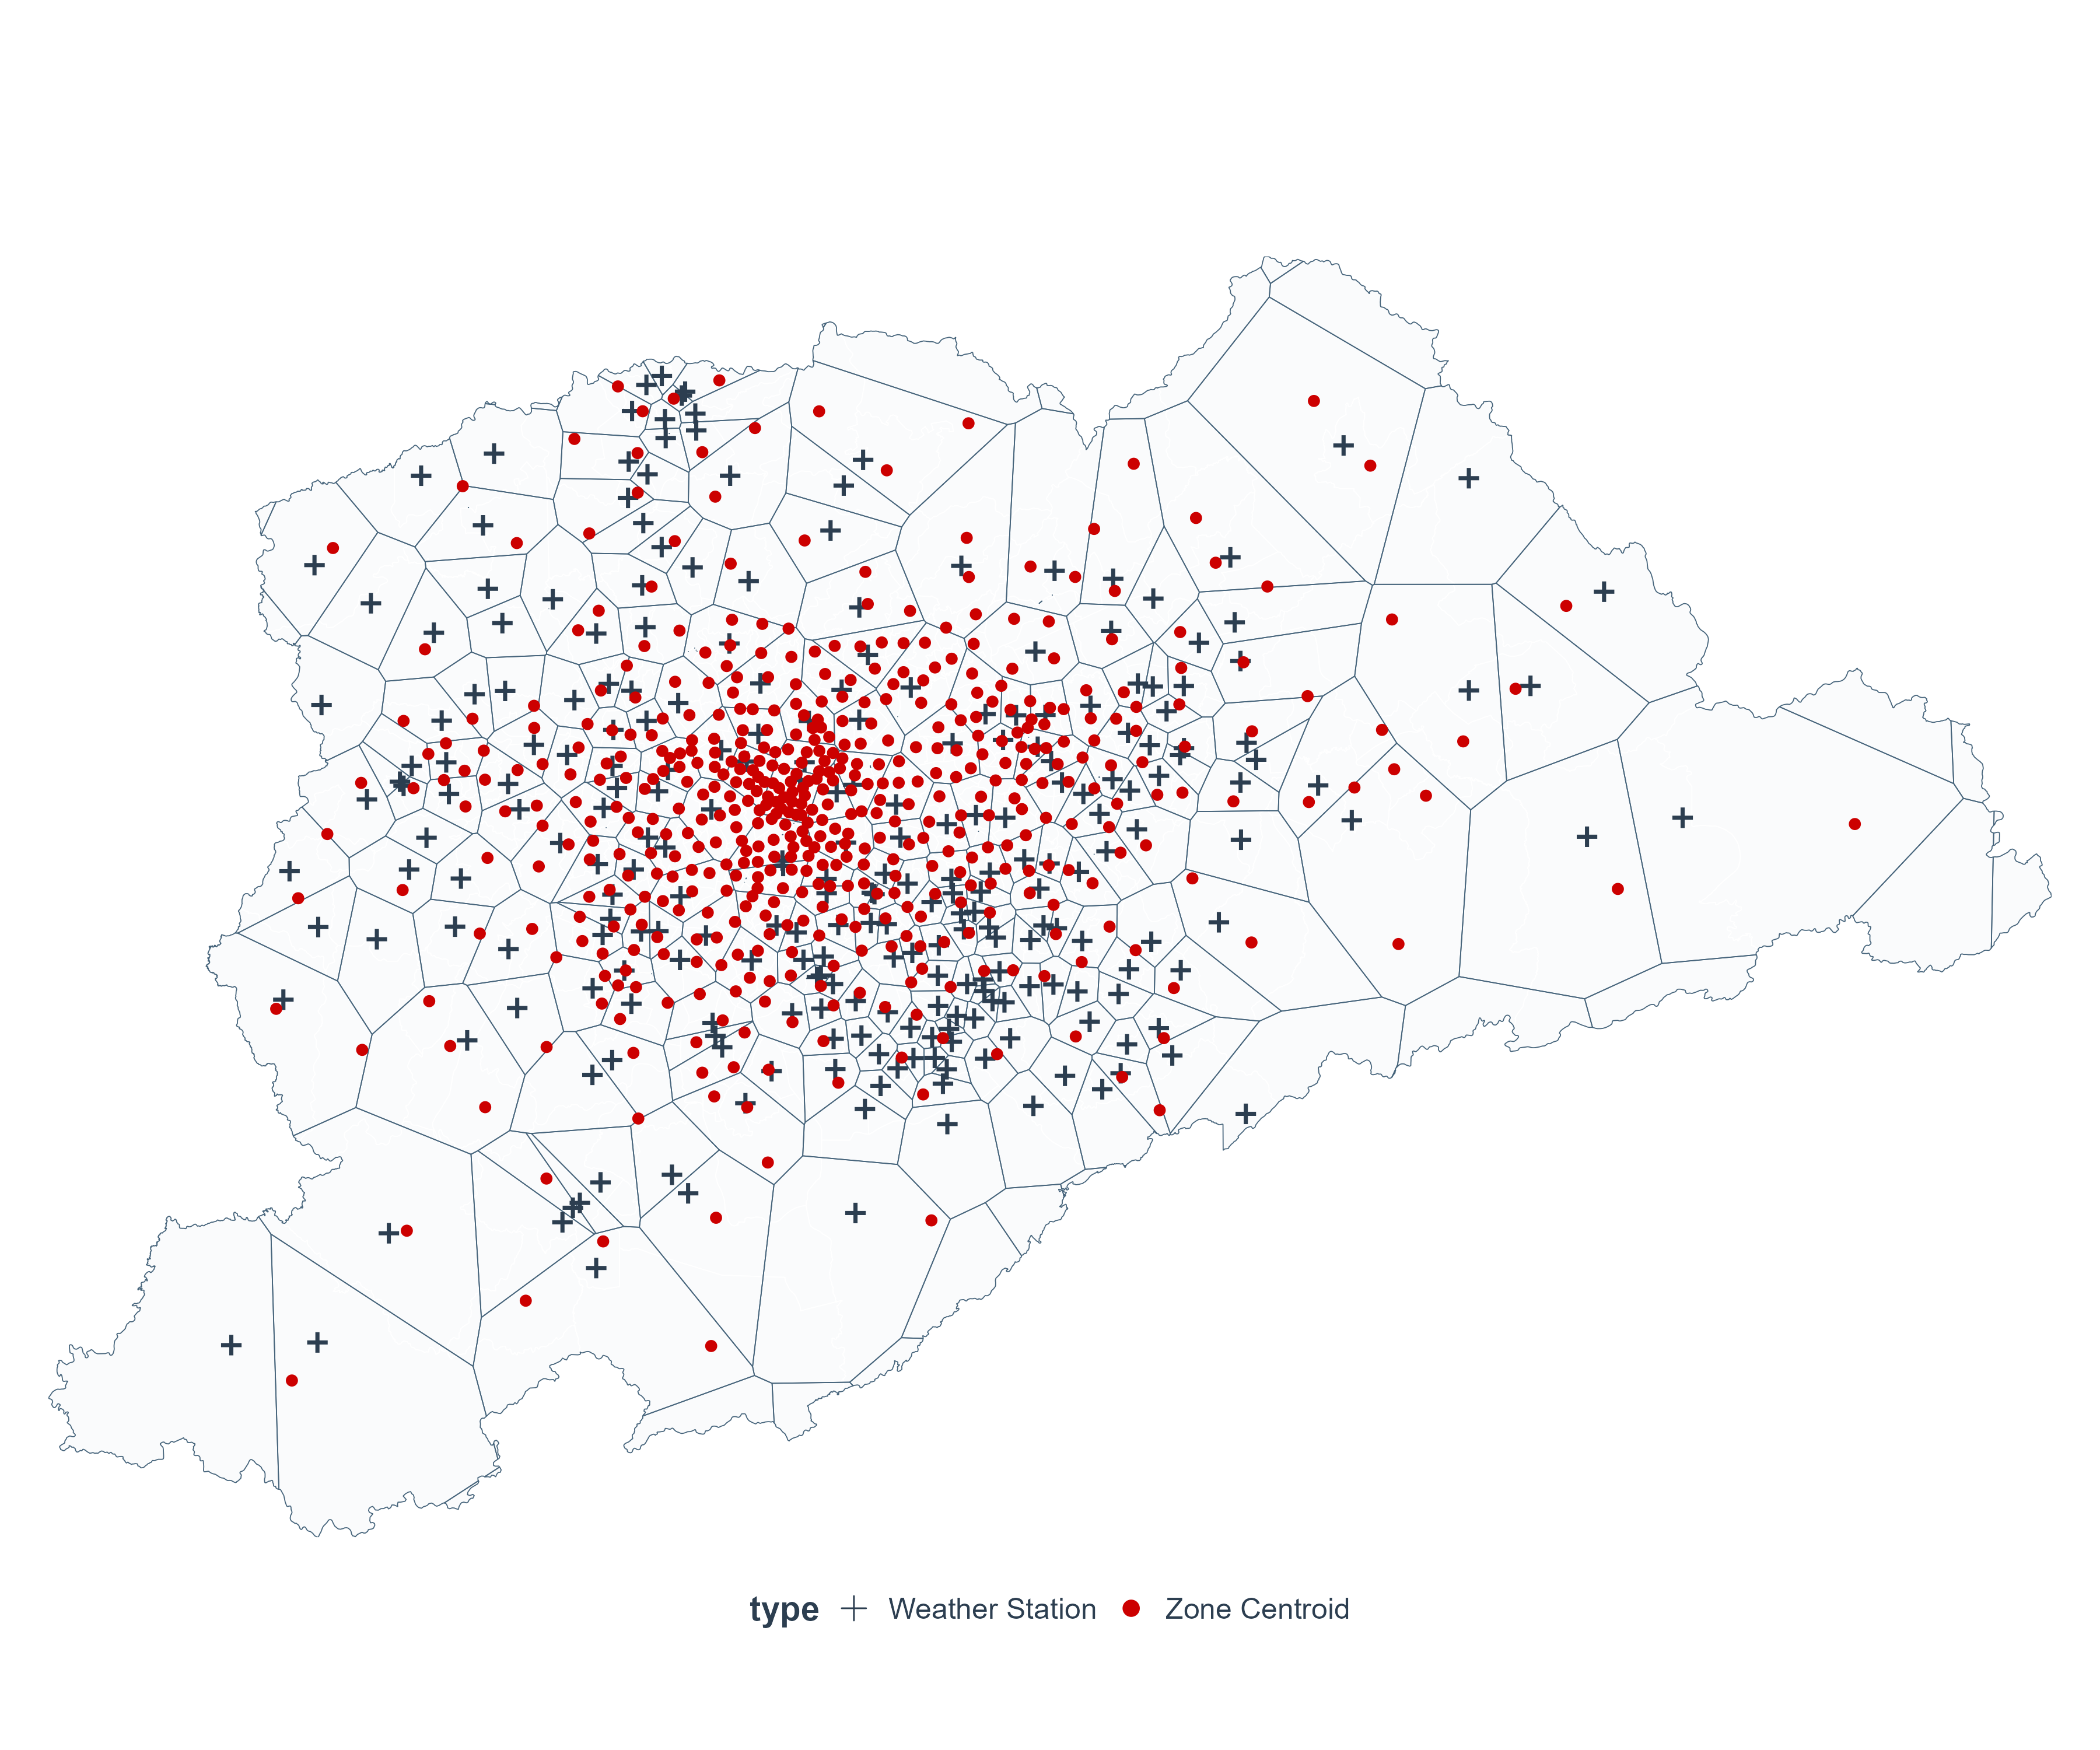
\includegraphics[width=0.8\textwidth]{../figures/rmsp_voronoi.png}
    \caption{Spatial representation of the RMSP region: (top) zone partitions, (bottom) Voronoi diagram illustrating spatial partitions based on centroid proximity to weather stations.}
    \label{fig:rmsp_voronoi}
\end{figure}
